Qt3D provides a high-level interface to OpenGL which allows us to display instrument components in 3D. Qt3D's entity framework is similar to other GUI frameworks and 3D engines such as Unity. This means all the textures, meshes, and transformations can be stored with a single entity in the Qt3D view. An important requirement of the NeXus Constructor is a feature for handling object translations. With Qt3D we can easily facilitate these changes without having to build the entire entity from scratch. 
\iffalse
\begin{figure}
\caption{Qt3D's element inspector}
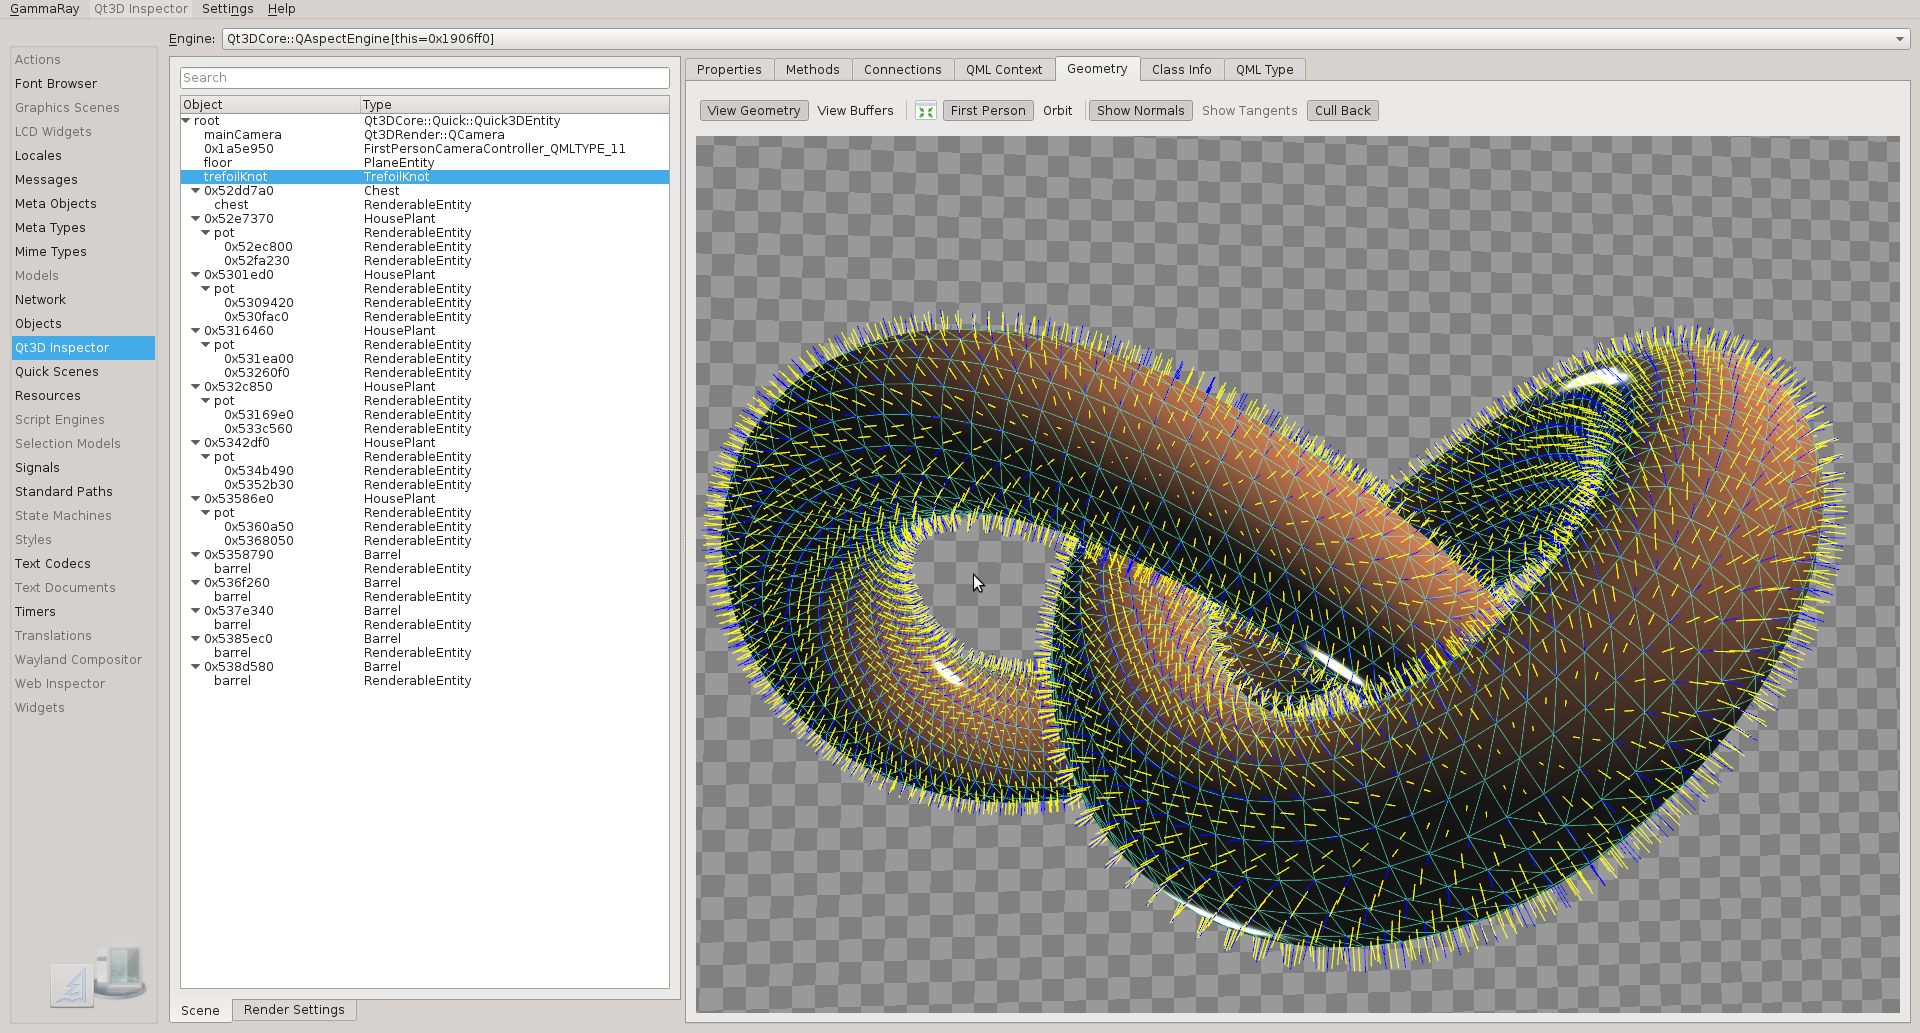
\includegraphics[width=\linewidth]{qt3d.png}
\end{figure}
\fi
\bigskip
